\section{FSM en descripción comportamental \label{sec:s2}}



\begin{center}
	\begin{minipage}{10cm}
		Describir por comportamiento la FSM del problema que está siendo considerado (como las
		descripciones vistas en clase). Indicar al compilador usar códigos del registro de estado en forma
		``minimal bits''. Compilar, simular y ver resultado en el visor RTL, ¿se genera el diagrama de
		estados y la tabla de códigos en los reportes?
		
		\enter
		
		Para indicar al compilador qué códigos del registro de estado debe usar se debe ir al menú de
		Quartus correspondiente: 
		
		\enter
		
		Assignments $>$ Settings $>$ Analysis $>$ sinthesis $>$ State Machine Processing
	\end{minipage}
\end{center}

\enter


Observando el diagrama RTL, se nota que la codificación de los estados de la
máquina da lugar a la interpretación de 2 componentes que representan el estado
actual y el estado siguiente (cosa que en VHDL se describiría de forma separada).
\begin{figure}[ht]
	\centering
	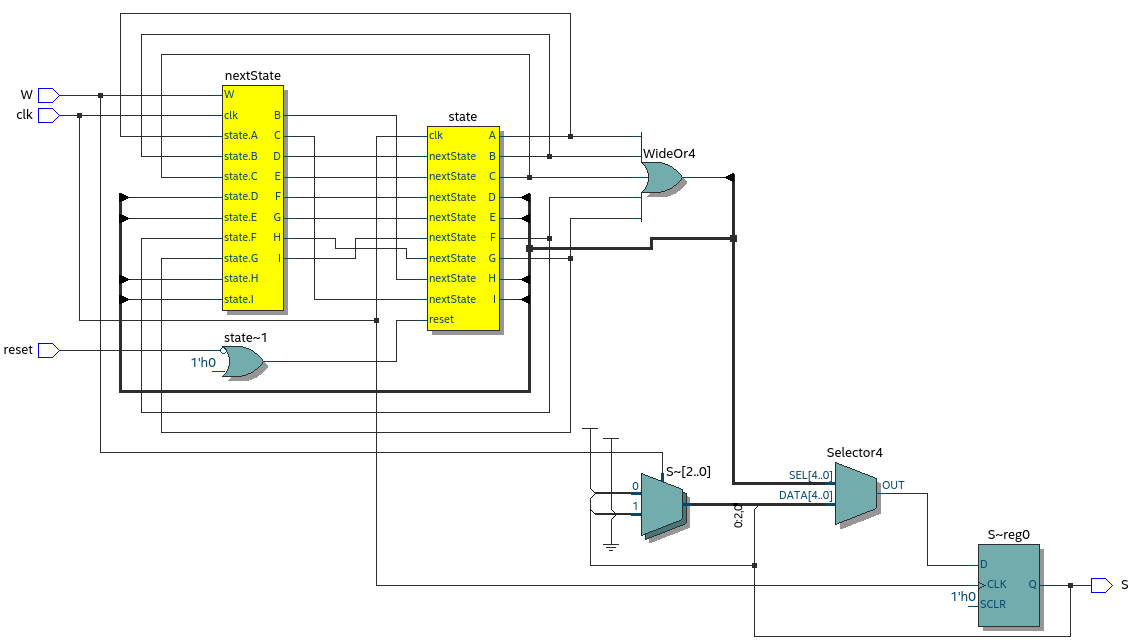
\includegraphics[scale=0.35]{fsmcom_1hot_rtl.png}
	\caption{
		Diagrama RTL de la FSM, usando \textit{minimal bits}.
		\label{fig:fsmcom_1hot_rtl}
	}
\end{figure}


Por otro lado, Observando la simulación, se aprecia un estado desconocido al inicio de dicha simulación, hasta 
que se tomen los valores del estado inicial y se comience el análisis, luego se valida cuando existen 4 consecutivos iguales.
\begin{figure}[ht]
	\centering
	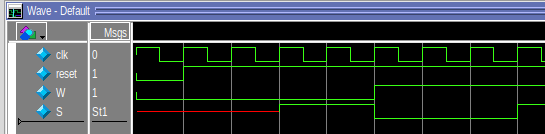
\includegraphics[scale=0.4]{fsmcom_1hot_sim.png}
	\caption{
		Simulación de la FSM, usando \textit{minimal bits}.
		\label{fig:fsmcom_1hot_sim}
	}
\end{figure}

\newpage

Cuando se analiza el reporte con la configuración de máquina de estados finitos
se aprecia la codificación de \textit{minimal bits} utilizada en la descripción,
al igual que una máquina que carece de conexiones.
\begin{figure}[ht]
	\centering
	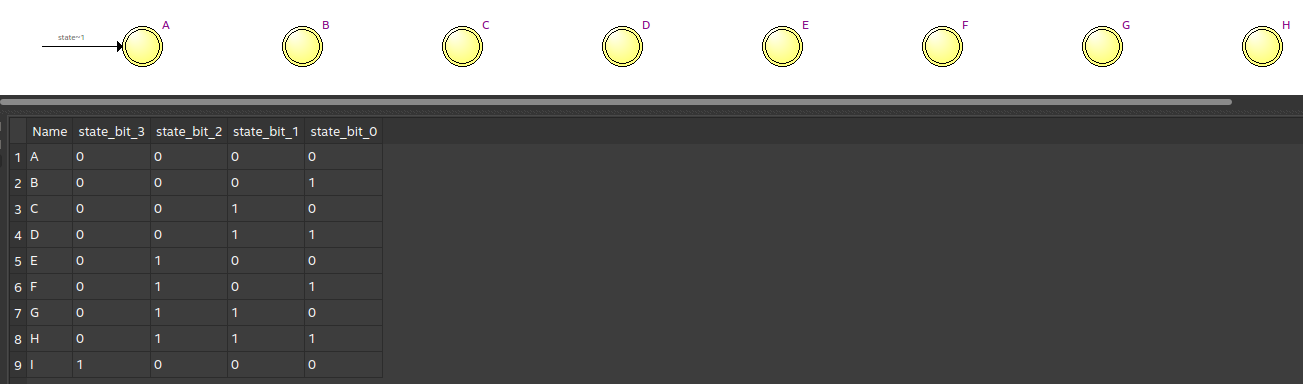
\includegraphics[scale=0.31]{fsmcom_min_state.png}
	\caption{
		Diagrama de estados para el estado actual, usando \textit{minimal bits}.
		\label{fig:fsmcom_min_state}
	}
\end{figure}

\enter

Además, se genera la máquina de estados conectada que es observable al consultar el componente del estado siguiente.
\begin{figure}[ht]
	\centering
	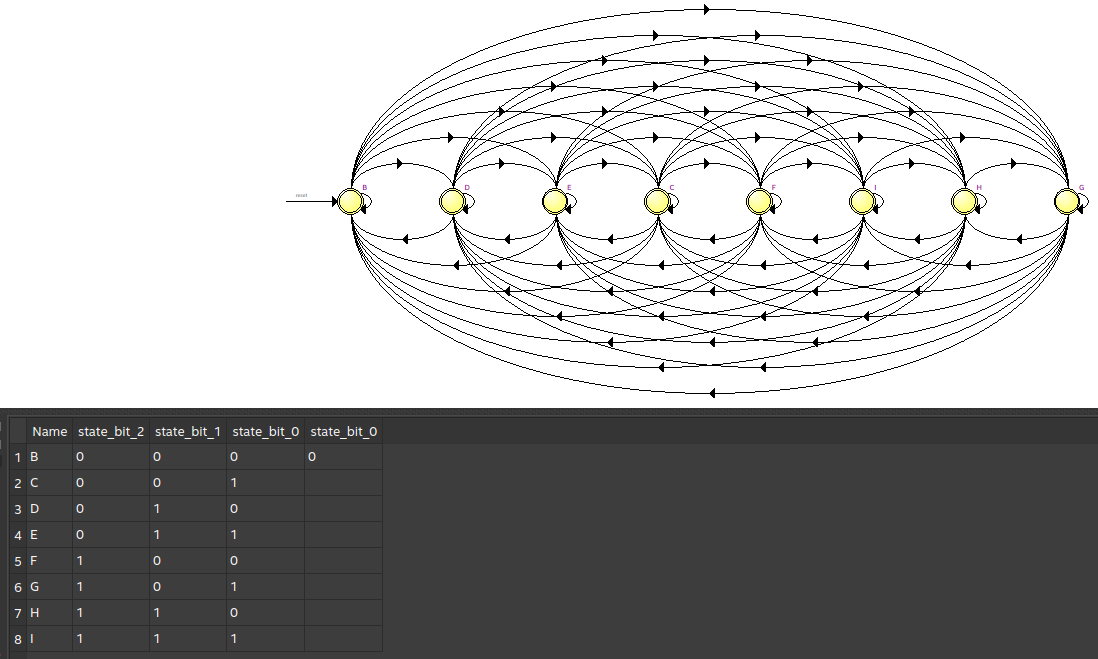
\includegraphics[scale=0.32]{fsmcom_min_nextstate.png}
	\caption{
		Diagrama de estados para el estado siguiente, usando \textit{minimal bits}.
		\label{fig:fsmcom_min_nextstate}
	}
\end{figure}








\clearpage
\begin{center}
	\begin{minipage}{10cm}
		Repetir el inciso 3 pero indicando codificación ONE - HOT. ¿Qué códigos ONE-HOT fueron
		utilizados, como los de la tabla normal o la modificada?
	\end{minipage}
\end{center}

\enter

En el caso del diagrama RTL y la simulación, se genera el mismo resultado que
el visto en la \autoref{fig:fsmcom_1hot_rtl} y \autoref{fig:fsmcom_1hot_sim}, 
respectivamente

\enter

Cuando se analiza el reporte con la configuración de máquina de estados finitos
se aprecia la codificación de \textit{one hot} \textbf{modificada}, esto porque el compilador busca implementarlo de una manera más óptima y para aeso sirve más esta codificación, porque se ahorra flip-flops.
\begin{figure}[ht]
	\centering
	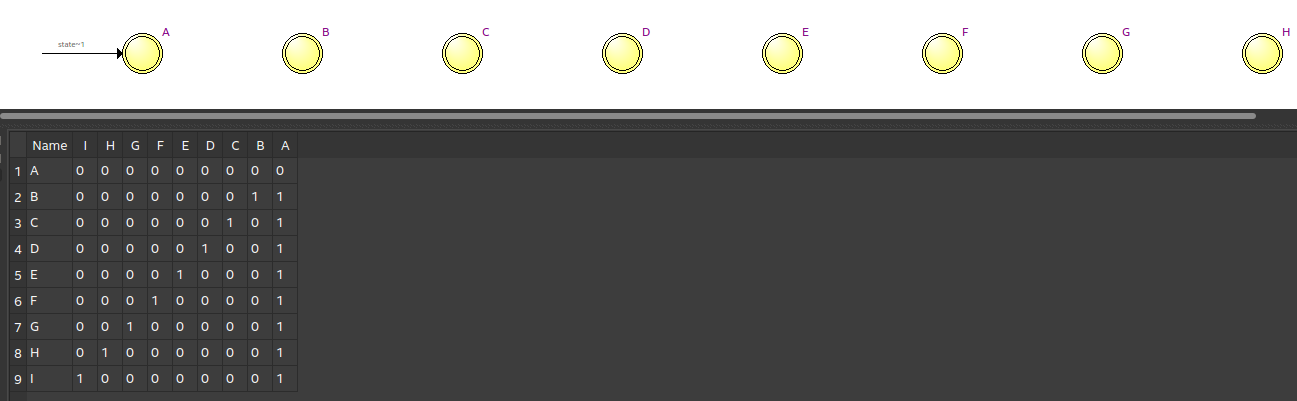
\includegraphics[scale=0.3]{fsmcom_1hot_state.png}
	\caption{
		Diagrama de estados para el estado actual, usando \textit{One Hot}.
		\label{fig:fsmcom_1hot_state}
	}
\end{figure}

Además, se genera la máquina de estados conectada, observable al consultar el componente del estado siguiente.
\begin{figure}[ht]
	\centering
	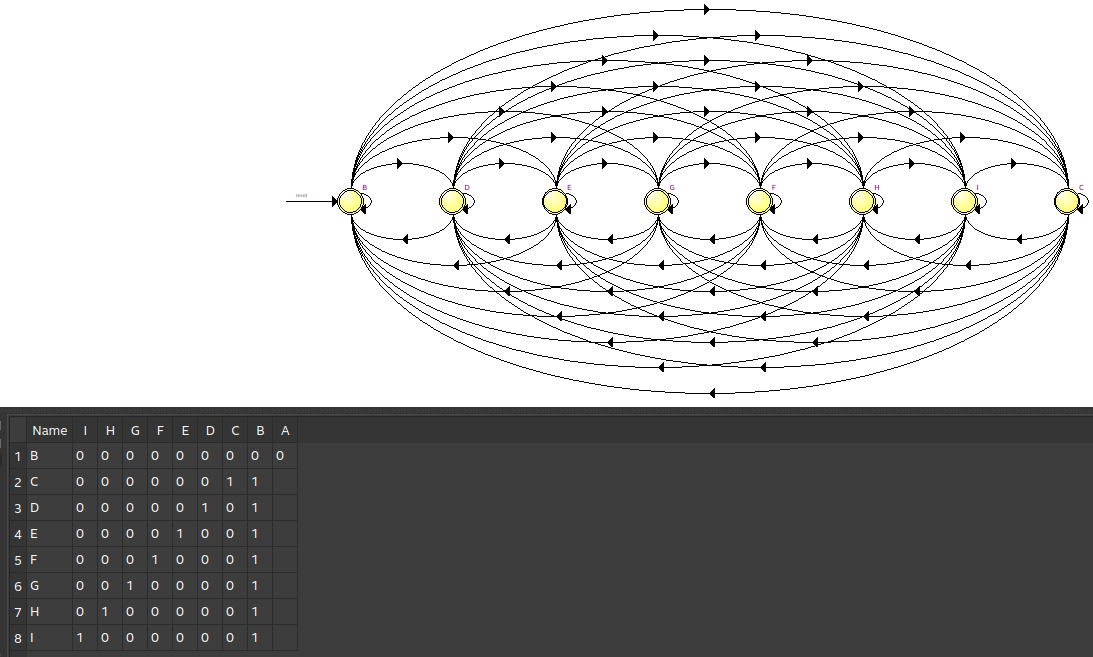
\includegraphics[scale=0.32]{fsmcom_1hot_nextstate.png}
	\caption{
		Diagrama de estados para el estado siguiente, usando \textit{One Hot}.
		\label{fig:fsmcom_1hot_nextstate}
	}
\end{figure}





